\chapter{Methodology}\label{sec:Chapter3-Methodology}

This methodology chapter serves to introduce strategies, implementations, models and approaches which are put into practice in the Experiments chapter (Chapter~\ref{sec:Chapter4-Results}). Therefore, it will include:
\begin{itemize}[itemsep=0.1cm]
    \item \textbf{Particle Swarm Optimization:} an explanation of the most important of the sampling techniques utilized in the experiments.
    \item \textbf{Custom Implementation of PSO:} a detailed description of the design of the custom implementation of the algorithm, and some insights on the actual code implementation.
    \item \textbf{Enhancing Optuna Optimization:} a description of the design of the infrastructure built to run the experiments, in order to make Optuna more robust and reliable, and the experiments more comparable.
    \item \textbf{Applied Neural Network Models:} contains the list, with attached descriptions, of the machine learning objects involved in the experiments, along with descriptions of the training and evaluation of the utilized models.
\end{itemize}

\myparagraph{Code Repository:}
All the implementation details listed throughout this chapter refer to the following repository: \cite{Repository-THESIS}.
The repository is divided into two main packages, \texttt{utils} and \texttt{experiments}.
\\[0.3cm]The \texttt{experiments} package contains the code for the execution of the actual experiments and additional “private” code which is specific for the execution of the determined experiment.
\\[0.3cm]The \texttt{utils} package contains code which is common to all the experiments, in order to make the project more maintainable and modularized.

\section{Particle Swarm Optimization}

\subsection{Introduction to Particle Swarm Optimization}

Particle Swarm Optimization (PSO) is an optimization approach originally proposed by Kennedy and Eberhart in 1995 \cite{Tesi-3.3}. The idea was to replicate the behaviour of certain animal species which moves in groups, such as flocks of birds or shoals of fish.
\\[0.3cm]The reason is the assumption that each singular individual in the group can take advantage from the collective experience of the entire group; basically, each individual can benefit from what it learns from other individuals, and in the same way, it can share its discoveries with the other individuals \cite{Tesi-3.1}.

\subsubsection{Particle Swarm Optimization as an Optimization Problem}

Translating the previous explained behaviour into specific terms, each individual can be interpreted as an agent which “flies” in the Search Space, where each physical position is a candidate solution in the n-dimensional Search Space, and the best solution found by the entire group is the best solution.
\\[0.3cm]The best solution found by the entire group is likely not the real global optimal solution. However, it is a solution that is near the global optimum.
% 
% \myparagraph{Formalization of Particle Swarm Optimization:}
\\[0.3cm]The goal of Particle Swarm Optimization, as all optimization problems, is to find value which maximizes (or minimizes) the value of an objective (or Fitness) function $f$.
\\[0.3cm]The Objective Function $f$ is defined on a Search Space {$\textbf{X}$}, the multi-dimensional vector representing all the possible solutions within the defined limits.
The PSO algorithm will return the vector $X$, which represents a single solution, which maximizes (or minimizes) the value of $f$.
% 
% \myparagraph{General Procedure of PSO:}
\\[0.3cm]To find the maximum (or minimum) of the Fitness function $f$, the best solution would be to perform an exhaustive search on all the possible solutions. However, this approach is too computationally expensive, and basically inapplicable to higher-dimensional spaces \cite{Tesi-3.1}.
\\[0.3cm]Therefore, in PSO, the same way as a flock of birds searches for food, moving in the air, the algorithm starts with a number of random points in the search space, which are called Particles, and has them look for an optimal value by roaming in random directions.
\\[0.3cm]At each atomic step, each Particle (individual) searches for its Local Optimal value, basing its research on both the current Local Optimum, and the current Global Optimum of the whole Swarm.
After a certain number of iterations, the maximum (or minimum) value found as the Global Optimum is considered the optimal value for the function $f$.

\subsubsection{Particle Swarm Optimization Algorithm}

At the start of each iteration, each Particle has a position $x_i(t)$ and a velocity $v_i(t)$.

\myparagraph{Update of Particles:}\label{sec:UpdateOfParticles-3.1.1}
At the subsequent iteration, the update function will update the position and velocity of a Particle in accordance with the following rules:
\begin{equation}
	v_i(t+1) = \alpha v_i(t) + \beta_1(x_i^{(local)}(t) - x_i(t)) + \beta_2(x^{(global)}(t) - x_i(t))
\end{equation}
\begin{equation}
	x_i(t+1) = x_i(t) + v_i(t)
\end{equation}
Parameter $\alpha$ represents an “inertia”, which decreases over time, that is when t increases.
\\[0.3cm]Parameters $\beta_1$ and $\beta_2$, are the weight assigned to the Local and Global “parts” respectively. They are usually chosen randomly at each step. They are called Cognitive Coefficient and Social Coefficient, respectively.
\\[0.3cm]Parameter  $x_i^{(local)}$  is the Local Memory of an individual (Particle), it represents the best coordinates in the Search Space visited by that individual. It is updated as follows:
\begin{equation}
	x_i^{(local)} = x_i(\arg \max f(x_i(u)))
\end{equation}
Parameter $x^{(global)}$ is the Global Memory of the Swarm, it represents the best coordinates in the Search Space visited by an individual in the Swarm, basically the best solution so far. It is updated as follows:
\begin{equation}
	x^{(global)}(t) = x_j^{(local)}(t)
\end{equation}
Whenever Local Optimum (for each Particle) and Global Optimum (for the whole Swarm) is found, the values of the two memories are updated.

\myparagraph{Advantages of PSO Algorithm:}
Differently from other more traditional optimization algorithms, PSO does not depend on the gradient of the objective function.
Basically, unlike Gradient Descent, the movement of a Particle does not depend on which direction is “uphill” or “downhill”, because the Particle is guided by Local Optimum and Global Optimum only.
\\[0.3cm]This advantage makes PSO algorithms suitable for problems which objective functions are non-differentiable. Thus, it is an algorithm appliable to a wider range of optimization problems.
Another advantage is that PSO is an “Embarrassingly Parallel” problem; a type of problem particularly easy to parallelize, as each particle can be updated in parallel.

\myparagraph{Visual Example of PSO:}
In the figure (Fig.~\ref{fig:figure-3.1.1}), it can be observed how the particles progressively converge towards the Global Optimum, which represents the best solution found by the whole Swarm.
\begin{figure}[t]
	\centering
	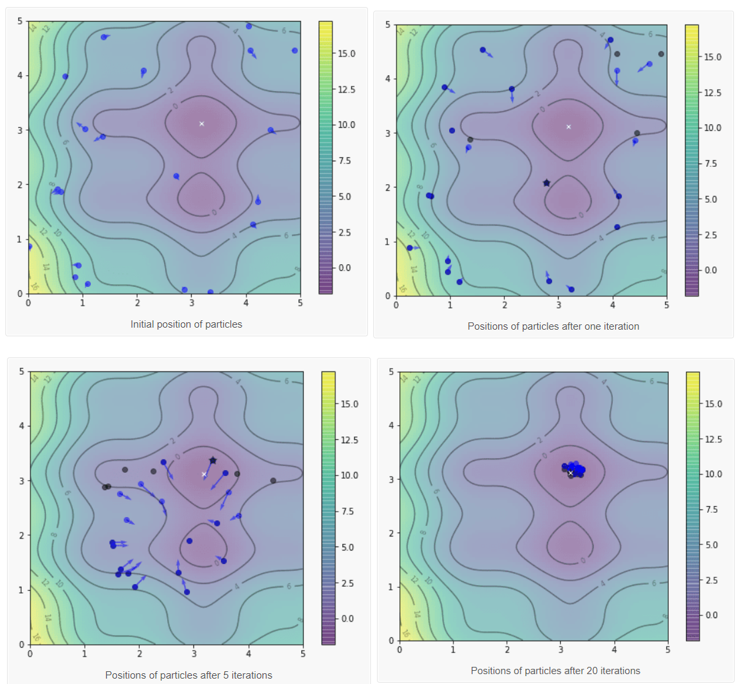
\includegraphics[width=14cm]{figures/figure-3.1.1.png}
	\caption[Visual Representation of Particle Swarm Optimization]{Visual representation of the convergence of the Particles to the Global Optimum in the Search Space in a Particle Swarm Optimization Algorithm. Source:~\cite{Tesi-3.1}}
	\label{fig:figure-3.1.1}
\end{figure}

\subsection{Components of Particle Swarm Optimization}

Particle Swarm Optimization can have better results, be faster and cheaper compared to other methods. It is an easy problem to parallelize. Does not require the target function to be differentiable. It has few and not very complex hyperparameters.
\\[0.3cm]In short, PSO has a large set of advantages; it is a modern solution to perform optimization tasks. The final objective remains the same as for every optimization problem: to minimize (or maximize) a given function.
\\[0.3cm]The three components of PSO algorithm are: Particle, Swarm and Optimization.

\subsubsection{Particle}

The Particle Swarm Optimization is inspired by the behaviour of flocks of birds. Therefore, the term “Particle”, refers to a single individual in the Swarm.
\\[0.3cm]Every Particle is defined by its Position and its Velocity in the Search Space.
The Position in the Search Space allows for the evaluation of the values corresponding to that position, whereas the Velocity allows Particles to move stochastically in the Search Space, in search of new better positions, and thus solutions.
% 
% \myparagraph{Initialization of Particles:}
\\[0.3cm]At the start of the optimization process, the positions of the Particles are defined randomly: random values of the Search Space are assigned to the Particles.
The Velocity and direction of the Particles are also randomly generated.
% 
% \myparagraph{Evaluation of Particles:}
\\[0.3cm]The Particle in the PSO is thus an agent, the position this agent has in the Search Space is a potential solution, a candidate solution.
Each Particle has Fitness values, which are evaluated by the Fitness Function, which is the function subject of the optimization.
The Fitness Function evaluates a Particle's Positions, taking in input the values of the Search Space corresponding to that position.

\subsubsection{Swarm}
The Swarm is the Population of Particles in the optimization process, it represents the flock of birds.
\\[0.3cm]PSO has similarities with Genetic Algorithms, but differently from them, there are no Evolution Operators to update the individual for the next generation.
In PSO the next generation of individuals is an update of the former generation, which Position and Velocity are updated in order to improve the Fitness.

\myparagraph{Inertia, Cognitive Intuition and Social Intuition:}
After each iteration in the Search Space, the Velocity of each Particle is stochastically accelerated; consequently, also its Position will change.
\\[0.3cm]The value the Velocity is going to be updated into is influenced by three factors: Inertia, Cognitive Intuition and Social Intuition. (Fig.~\ref{fig:figure-3.1.2})
\\[0.3cm]Inertia is the tendency to keep the Velocity from the previous iteration.
Cognitive Intuition is what makes the Particle accelerate toward the previous best Local Position, which is the best Position (corresponding to best Fitness) that Particle has achieved so far.
Social Intuition is what makes the Particle accelerate toward the previous best Global Position, which is the best Position (corresponding to best Fitness) the Particles in the Swarm have achieved so far.
\begin{figure}[t]
	\centering
	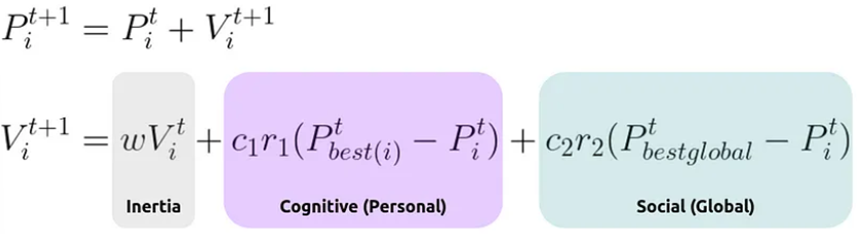
\includegraphics[width=13cm]{figures/figure-3.1.2.png}
	\caption[Alternative Update Functions for PSO]{Alternative update functions for the Velocity of the Particles in a Particle Swarm Optimization Algorithm, where the three components of the update function are represented, and additional parameters, $c_1$ and $c_2$ are introduced. Source:~\cite{Tesi-3.2}}
	\label{fig:figure-3.1.2}
\end{figure}

\subsubsection{Optimization}

The Optimization component of PSO, consists in the actual process of updating the parameters, with the correlated setting of Hyperparameters.
Inertia, Cognitive and Social coefficients have the function to control the levels of Exploitation and Exploration.
\\[0.3cm]Exploitation means using the good solutions found so far in order to search for even better solutions in that mathematical neighbourhood. Exploration means to explore distant sections of the Search Space, in search of new information on the Space or potentially improving solutions.
% 
% \myparagraph{Weighting of Acceleration:}
\\[0.3cm]At each iteration, both the Cognitive section and the Social section of the update formula are weighted by random terms \cite{Tesi-3.2} \cite{Tesi-3.5}.
Basically, Cognitive acceleration and Social acceleration are stochastically adjusted by weights to make the update process more random and less deterministic. The possible values that the coefficients can assume are in Fig.~\ref{fig:figure-3.1.3}.
\begin{figure}[t]
	\centering
	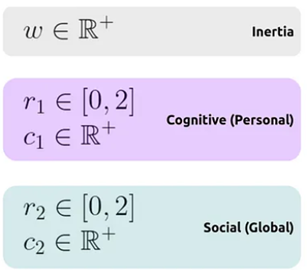
\includegraphics[width=5cm]{figures/figure-3.1.3.png}
	\caption[Values Ranges for PSO Parameters]{Ranges of values for the Parameters of a Particle Swarm Optimization Algorithm. Source:~\cite{Tesi-3.2}}
	\label{fig:figure-3.1.3}
\end{figure}
% 
% \myparagraph{Value of Inertia:}
\\[0.3cm]The value of the Inertia coefficient defines the ability of the Swarm to change direction.
Lower values of Inertia coefficient lead to better convergence; so low Inertia increases the exploitation of the best solutions.
Higher values of Inertia coefficient increase the exploration around the best solutions.
Values too high for Inertia, values $>1$, cause divergence of the Particles \cite{Tesi-3.2}.
% 
% \myparagraph{Value of Cognitive Coefficient:}
\\[0.3cm]The value of Cognitive coefficient defines the ability of the Swarm to be influenced by the personal solutions of each Particle.
If the Cognitive coefficient is too high, then there will be no convergence, as each individual would be too focused on its optimal solution \cite{Tesi-3.2}.
% 
% \myparagraph{Value of Social Coefficient:}
\\[0.3cm]The value of Social coefficient defines the ability of the Swarm to be influenced by the best global solutions of the whole Swarm.

\myparagraph{Auto Hyperparameters:}
Inertia, Cognitive and Social coefficients are all three Hyperparameters for the optimization process of PSO.
\\[0.3cm]Searching for the optimal values of their coefficient is a complex and expensive task, as it would require another optimization process.
Moreover, the optimal value of these parameters changes during the optimization process, as the iterations go on.
\\[0.3cm]Therefore, a satisfactory solution is to update the coefficients over the iterations \cite{Tesi-3.2}.
Good recommended update formulas, coming from empirical studies, are the equations below.
\\[0.3cm]The initial values should guarantee high exploration and more individuality, so high Inertia and Cognitive and low Social.
\\[0.3cm]Toward the end of the optimization, values should guarantee high exploitation and convergence to the local optimum, so low Inertia and Cognitive and high Social.
\begin{equation}
	w = 0.4\frac{(t-N)}{N^2} + 0.4
\end{equation}
\begin{equation}
	c_1 = -3\frac{t}{N} + 3.5
\end{equation}
\begin{equation}
	c_2 = +3\frac{t}{N} + 0.5
\end{equation}

\subsection{Principles, Applications and Variants of PSO}

This subsection, will examine: Principles of Swarm Intelligence, real-world applications of Particle Swarm Optimization, and PSO variants.

\subsubsection{Principles of Particle Swarm Optimization}

Particle Swarm Optimization has evolved a lot during its first experimental phase.
While it was originally meant to simulate the behaviour of a flock of birds, the final form of the algorithm resembles more of a Swarm than a flock. For this reason, it took the name of Swarm Optimization.
\\[0.3cm]The first researcher who talked about Swarm Intelligence, Millonas \cite{SwarmIntelligence}, defined five principles of Swarm Intelligence.
Particle Swarm Optimization adheres to all five principles.
\begin{enumerate}[itemsep=0.1cm]
    \item \textbf{Proximity Principle:} “The population should be able to perform simple space and time computations”.
	\item \textbf{Quality Principle:} “The population should be able to respond to quality factors in the environment”.
	The PSO adheres to this principle because the population, the Swarm, tends to follow the two positions Local Optimum and Global Optimum, which are the environment's factors.
	\item \textbf{Diverse Response Principle:} “The population should ensure enough diversity in its responses”.
	The PSO adheres to this principle because the responses range from the Local Optimum of the Particle and the Global Optimum of the Swarm, ensuring the diversity.
	\item \textbf{Stability Principle:} “The population should not change its behaviour at each environmental change”.
	The PSO adheres to this principle because the population only changes when the Global Optimum is updated and is therefore stable.
	\item \textbf{Adaptability Principle:} “The population should be able to change its behaviour when it is worth the computational price”.
	The PSO adheres to this principle because the population does change its behaviour when the Global Optimum is updated.
\end{enumerate}
% 
% \myparagraph{1 - Proximity Principle:}
% The population should be able to perform simple space and time computations.
% 
% \myparagraph{2 - Quality Principle:}
% The population should be able to respond to quality factors in the environment.
% \\[0.3cm]The PSO adheres to this principle because the population, the Swarm, tend to follow the positions Local Optimum and Global Optimum, which are the environment's factors.
% 
% \myparagraph{3 - Diverse Response Principle:}
% The population should ensure enough diversity in its responses.
% \\[0.3cm]The PSO adheres to this principle because the responses range from the Local Optimum of the Particle and Global Optimum of the Swarm, ensuring the diversity.
% 
% \myparagraph{4 - Stability Principle:}
% The population should not change its behaviour at each environmental change.
% \\[0.3cm]The PSO adheres to this principle because the population only changes when the Global Optimum is updated and is therefore stable.
% 
% \myparagraph{5 - Adaptability Principle:}
% The population should be able to change its behaviour when it Is worth the computational price.
% \\[0.3cm]The PSO adheres to this principle because the population does change its behaviour when the Global Optimum is updated.

\subsubsection{Applications of Particle Swarm Optimization}

One of the main reasons why Particle Swarm Optimization is widely used as optimization technique, is that it is well-suited to a wide range of problems \cite{Tesi-3.4}.
The advantage of PSO is that it has a small number of Hyperparameters to set, this allow the algorithm to be easily appliable to specific applications \cite{Tesi-3.4} \cite{Tesi-3.1} \cite{Tesi-3.3} \cite{Tesi-3.5}.
\begin{itemize}[itemsep=0.1cm]
    \item \textbf{Evolution of Neural Networks:} Particle Swarm Optimization can substitute traditional methods for the optimization of a Neural Network's weights.
	PSO is able to reach or outperform traditional approaches like Backpropagation.
	PSO can work so well with Neural Networks, that it can not only be used to optimize the networks' weights, but also their structure. PSO is effective for any network architecture \cite{Tesi-3.4}.
	\item \textbf{Human Tremor Diagnosis:} PSO has been used in combination with Neural Networks for the diagnosis of Humar Tremor conditions, for example, Parkison's Disease \cite{Tesi-3.4}.
	\item \textbf{End Milling Manufacturing:} PSO has been used in combination with Neural Networks for End Milling manufacturing \cite{Tesi-3.4}.
	\item \textbf{Voltage Stability:} PSO has been used for dynamic power and voltage control in a Japanese electric establishment \cite{Tesi-3.4}.
	\item \textbf{Determination of Battery State:} PSO has been used in combination with Neural Networks for estimating the state-of-charge of electrical or hybrid vehicles \cite{Tesi-3.4}.
\end{itemize}
% \\[0.3cm]\textbf{Evolution of Neural Networks:} Particle Swarm Optimization can substitute traditional methods for the optimization of a Neural Network weights.
% PSO is able to reach or outperform traditional approaches like Backpropagation.
% PSO can work so well with Neural Networks, that not only can be used to optimize the networks' weights, but also their structure. PSO applies is effective for any network architecture \cite{Tesi-3.4}.
% \\[0.3cm]\textbf{Human Tremor Diagnosis:} PSO has been used in combination with Neural Networks for the diagnosis of Humar Tremor conditions, for example Parkison's Disease \cite{Tesi-3.4}.
% \\[0.3cm]\textbf{End Milling Manufacturing:} PSO has been used in combination with Neural Networks for End Milling manufacturing \cite{Tesi-3.4}.
% \\[0.3cm]\textbf{Voltage Stability:} PSO has been used for a dynamic power and voltage control in a Japanese electric establishment \cite{Tesi-3.4}.
% \\[0.3cm]\textbf{Determination of Battery State:} PSO has been used in combination with Neural Networks for estimating the state-of-charge of electrical or hybrid vehicles \cite{Tesi-3.4}.

\subsubsection{Variants of Particle Swarm Optimization}

The Particle Swarm Optimization is a popular and effective optimization technique; therefore, many variants of the approach have been developed \cite{Tesi-3.2}.
\\[0.3cm]Variants primarily focus on adding evolutionary capabilities to PSO or improving performance with Hyperparameters.
\begin{itemize}[itemsep=0.1cm]
    \item \textbf{Hybrid of Genetic Algorithm and PSO (GA-PSO):} implements the main aspects of GA approach, such as the capability of breeding and crossover.
    \item \textbf{Hybrid of Evolutionary Programming and PSO (EPSO):} implements the tournament selection in PSO, where the losing Particles change their position.
    \item \textbf{Adaptive PSO (APSO):} applies Fuzzy Logic to the Inertia coefficient. In addition, uses another PSO to perform the Hyperparameter Optimization for the first PSO.
    \item \textbf{Multi Objective PSO (MOPSO):} implements the concept of Pareto Dominance to determine which Particle should set the Global Optimum \cite{Tesi-3.5}.
    \item \textbf{Discrete PSO (DPSO):} makes the performance of optimization better, for example using a mixed-search approach \cite{Tesi-3.5}.
\end{itemize}
% 
% \myparagraph{Hybrid of Genetic Algorithm and PSO (GA-PSO):}
% Hybrid of Genetic Algorithm and PSO (GA-PSO) implements the mainly aspects of GA approach as the capability of breeding and crossover.
% 
% \myparagraph{Hybrid of Evolutionary Programming and PSO (EPSO):}
% Hybrid of Evolutionary Programming and PSO (EPSO) implements the tournament selection in PSO, where the losing Particles changes their position.
% 
% \myparagraph{Adaptive PSO (APSO):}
% Adaptive PSO (APSO) applies Fuzzy Logic to the Inertia coefficient. In addition, uses another PSO to perform the Hyperparameter Optimization for the first PSO.
% 
% \myparagraph{Multi Objective PSO (MOPSO):}
% Multi Objective PSO (MOPSO) implements the concept of Pareto Dominance to determine which Particle should set the Global Optimum \cite{Tesi-3.5}.
% 
% \myparagraph{Discrete PSO (DPSO):}
% Discrete PSO (DPSO) makes the performance of optimization better, for example using mixed search approach \cite{Tesi-3.5}.

\section{Custom Implementation of PSO}\label{sec:CustomImplementationOfPSO-3.2}

Particle Swarm Optimization, as described in the last section, is a powerful and successful Optimization algorithm, that can also be applied to HPO.
In the last few years, many libraries for PSO have been developed, for instance, PySwarm, which is probably the most popular.
\\[0.3cm]The problem with these libraries, as for the objectives of the experiments, is that they are hardly customizable, and often lack in explainability, making them less adaptable to HPO.
While this problem of explainability is potentially fixable, without being able to customize the original algorithm, the experiments would not be scientifically comparable between the ones run using Optuna's samplers.
\\[0.3cm]Therefore, two potential solutions are proposed so as to apply PSO to an HPO problem: the first was to implement from scratch a PSO algorithm that follows the same style as Optuna so that the two would be comparable; the second was to implement an Optuna Sampler with PSO.
The implementation of an Optuna Sampler with PSO will be discussed in the next section. In this section it will be examined the design of the PSO algorithm from scratch.
\\[0.3cm]All the code mentioned in this section refers to the package\newline\texttt{/experiments/PSO\_experiment/backend/} of the code repository \cite{Repository-THESIS}.

\subsection{High-Level Design}

The components of the algorithm are divided into five Python files: \texttt{PSO.py},\newline\texttt{pso\_pruners.py}, \texttt{pso\_runner.py}, \texttt{pso\_train\_utils.py} and \texttt{pso\_utils.py}.
These code files contain only what the algorithm needs to work, meaning that they do not contain the actual code of the experiments. In fact, the algorithm code is designed to mimic the functioning of Optuna, so that the same code to set up the Optuna experiments can be used to set up and perform experiments with this implementation of PSO. (Class Diagram in Fig.~\ref{fig:figure-3.2.1})
% 
% \myparagraph{Contents of the Main Code Files:}
\\[0.3cm]The contents and purpose of the main code files are the following:
\begin{itemize}[itemsep=0.1cm]
    \item \texttt{PSO.py}: is the main file of the package, the actual core of the algorithm. It contains the \texttt{PSO} and \texttt{Particle} classes, together with some other private code.
    \item \texttt{pso\_pruners.py}: contains the definition of the Pruners of the mini library. At the current state there is only one implemented Pruner which is the Median Pruner. It mimics the functioning of Optuna's Pruners.
    \item \texttt{pso\_runner.py}: contains the definition of the \texttt{PSORunner} class, which is a wrapper of the optimization process that manages potential errors, logging, and saving of the results.
    \item \texttt{pso\_train\_utils.py}: contains the train loop function which should be used inside the objective function of the optimization process. It also contains some other private code.
    \item \texttt{pso\_utils.py}: contains some constants and utility functions, in particular the one applied to encode and decode the value of the Hyperparameters from “internal” to “external” representations and vice-versa.
\end{itemize}
\begin{figure}[t]
	\centering
	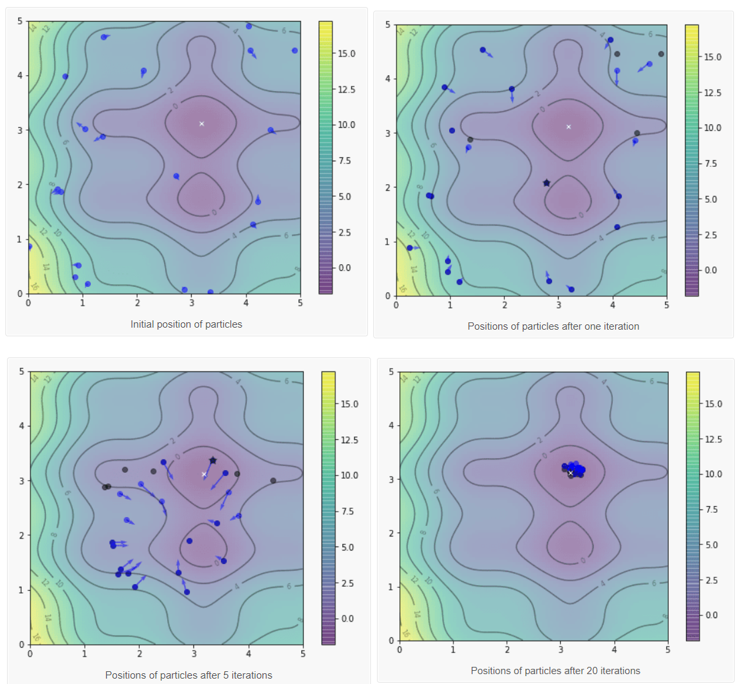
\includegraphics[width=15cm]{figures/figure-3.2.1.png}
	\caption[Class Diagram of Custom PSO Implementation]{Class Diagram of the custom implementation of the Particle Swarm Optimization with the related support code.}
	\label{fig:figure-3.2.1}
\end{figure}

\subsection{Components of the PSO Algorithm}

The true core of the algorithm, contained in \texttt{PSO.py}, consists of three fundamental components, which are: \texttt{Particle}, \texttt{PSOTrial} and \texttt{PSO}.

\subsubsection{Particle}

The \texttt{Particle} class is the representation of the concept of “Particle” in the original PSO algorithm.
% 
% \myparagraph{Attributes:}
\\[0.3cm]In this specific implementation, the Particle has the following attributes: \texttt{paticle\_id}, \texttt{position}, \texttt{velocity}, \texttt{personal\_best\_position}, \texttt{personal\_best\_score}.
The position and the velocity of the particle are initialized with randomly generated arrays.
% 
% \myparagraph{Methods:}
\\[0.3cm]The particle has two methods, which are \texttt{update\_velocity()} and \texttt{update\_position()}. 
The version of the strategy for the velocity update is the one with the Cognitive and the Social coefficients ($c_1$ and $c_2$). The random coefficients ($r_1$ and $r_2$) are chosen randomly, whereas, the other two coefficients, together with the Inertia coefficient ($w$), are passed as an input.
The strategy for the position update is the standard one, with the exception that values which go outside the Search Space are clipped (approximated to the nearest bound value).

\subsubsection{PSOTrial}

The \texttt{PSOTrial} class, as the name suggests, is a representation of a trial during the optimization. Its functioning is inspired by the \texttt{Trial} object of Optuna.
Its main objective is to carry metadata regarding each trial of the optimization process, so as to the results can be displayed the same way they are in Optuna.
% 
% \myparagraph{Attributes:}
\\[0.3cm]The \texttt{PSOTrial} object has the following attributes: \texttt{particle\_id}, \texttt{generation}, \newline\texttt{hyperparameters}, \texttt{datetime\_start}, \texttt{datetime\_complete}, \texttt{duration}, \texttt{score}, \texttt{state}, \texttt{user\_attrs}, \texttt{is\_pruned}, \texttt{pruner}, \texttt{last\_reported\_step}, \texttt{best\_reported\_score}.
The last four attributes are related to the pruning system. The \texttt{user\_attrs} attribute is a map object which allows the user to set custom metadata in the trial, like it can be done in Optuna. The other attributes are self-explainatory.
% 
% \myparagraph{Methods:}
\\[0.3cm]The methods realize functionalities such as completion of a trial, conversion to map, setters, and functions related to pruning.

\subsubsection{PSO}

The \texttt{PSO} class is the representation of the actual PSO algorithm. It is designed to be equivalent to a \texttt{Study} object of Optuna.
One instance of the \texttt{PSO} class carries on a whole optimization process, in the same way as an instance of Optuna's \texttt{Study} instance.
% 
% \myparagraph{Attributes:}
\\[0.3cm]The attributes of the \texttt{PSO} class are the following:
\begin{itemize}[itemsep=0.1cm]
    \item \texttt{objective\_function}: the objective function of the HPO process, to be passed at the initialization of the object just like in Optuna.
    \item \texttt{bounds}: is a 2D array which contains the lower bounds and the upper bounds of each non-categorical hyperparameter.
    \item \texttt{hps}: contains the mapping between the hyperparameter name and the index inside the inner arrays of bounds.
    \item \texttt{num\_particles}: is a hyperparameter of the algorithm itself; it represents the number of Particles in the Swarm.
    \item \texttt{max\_generations}: is another hyperparameter of the algorithm itself; it represents the maximum number of iterations (Generations) of the algorithm.
    \item \texttt{pruner}: the Pruner object to use in the algorithm.
    \item \texttt{pso\_stopper}: must be an \texttt{PSOStopper} object, which is another secondary class defined in the file. It Early-Stops the process according to a specified Tolerance and Patience.
    \item \texttt{swarm}: is the representation of the concept of Swarm. Rather than creating a specific class for it, it simply is a list of Particles (list of \texttt{Particle}).
    \item \texttt{global\_best\_score}: the best score at any given point in time.
    \item \texttt{global\_best\_position}: array which values represent the coordinates in the Search Space for the best position at any given point in time.
    \item \texttt{trials\_list}: list of all the \texttt{PSOTrial} objects.
    \item \texttt{best\_trial}: initialized at the end of the optimization, stores the best trial.
\end{itemize}
%
% \myparagraph{Methods:}
The methods of the \texttt{PSO} class, excluding the private or less important methods, are the following: \texttt{optimize()}, \texttt{inertia\_factor\_update()}, \texttt{cognitive\_factor\_update()}, \texttt{social\_factor\_update()}.
The three update methods are implemented using the formulas explained in the Particle Swarm Optimization section (Sec.~\ref{sec:UpdateOfParticles-3.1.1}).
\\[0.3cm]The \texttt{optimize()} method is where the actual PSO algorithm takes place. Here is where the optimization loop happens. The first level loop iterates over the maximum number of generations, then the inner loop iterates over each particle of the swarm.
After the particle is evaluated during a determined generation, and thus in a determined position, two checks are made to determine if the current result is better than the local and global better results.
Finally, at the end of a generation, each particle is updated using its update methods, with the values for $w$, $c_1$ and $c_2$ obtained from the three update methods mentioned earlier.
At the end of the whole loop, the method ends, returning the best global hyperparameters and the best global score.

\section{Enhancing Optuna Optimization}\label{sec:EnhancingOptuna-3.3}

Hyperparameter Optimization is expensive, and tools like Optuna not only exist to make the process more efficient but also to simplify the setup of the optimization.
Nevertheless, especially when the experiments grow in complexity, even tools like Optuna start to show weaknesses and robustness problems.
\\[0.3cm]Therefore, it is necessary to use Optuna to its full potential, gaining advantage from its additional abilities, such as the Storage. Moreover, an infrastructure beyond Optuna is also necessary to handle error throwing and to make persistent the data that Optuna Storage does not memorize.
\\[0.3cm]These extras are not always easy to setup, or at least require a setup for each Study. This, added to the already present normal setup of the Study, with the creation of the object and the launch of the optimization, makes the Study initialization process very heavy.
This would be perfectly fine in normal circumstances, but the goal of the proposed experiments, is to compare the different optimization techniques and sampling algorithms, thus, the previously described workflow should be repeated for each Study.
\\[0.3cm]The solution is to abstract some functionalities of Optuna, basically wrapping them, so as to reduce the quantity of code to write and improve the performance and reliability of the processes. (Object Diagram in Fig.~\ref{fig:figure-3.3.1})
\\[0.3cm]All the code mentioned in this section refers to the package \texttt{/utils/} of the code repository \cite{Repository-THESIS}.
\begin{figure}[t]
	\centering
	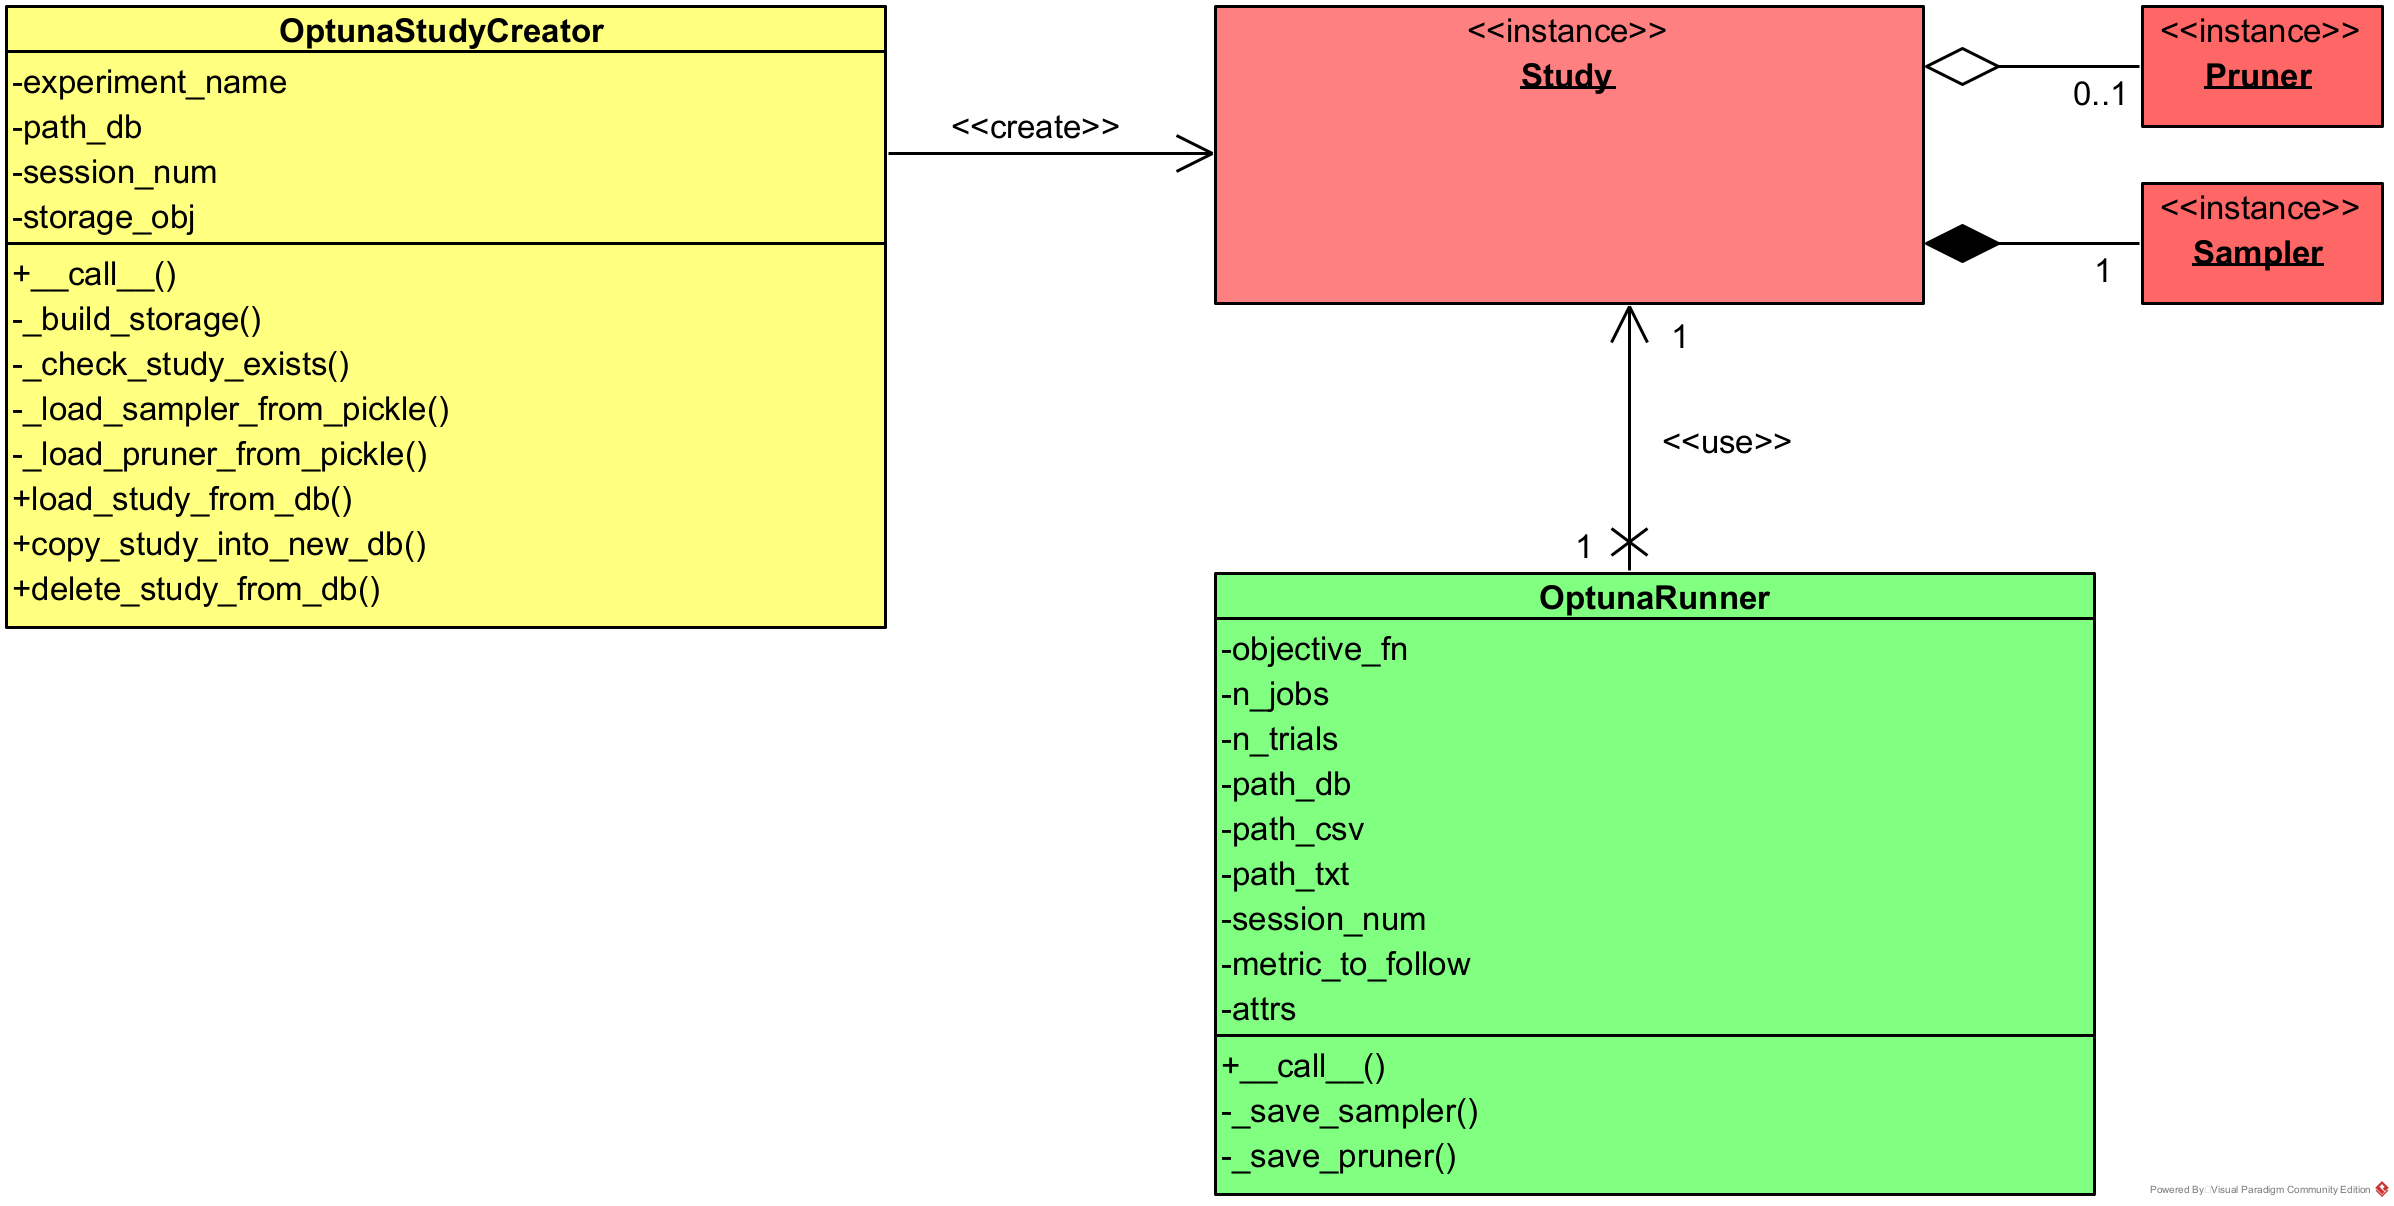
\includegraphics[width=15cm]{figures/figure-3.3.1.png}
	\caption[Object Diagram of Optuna Wrapping]{Object Diagram of the “wrapping”, or enhancement, of Optuna functionalities.}
	\label{fig:figure-3.3.1}
\end{figure}

\subsection{Optuna Wrapping}

The two main concerns relative to the abstraction of Optuna's functionalities are the initialization of the Study and the running of the optimization.
The proposed infrastructure, which wraps those two functionalities, has various objectives: to implement persistency (for both Optuna and additional metadata such as logs), to handle errors, to save the execution state of samplers and pruners (which Optuna does not do natively), to log and save the results in various formats, and other capabilities (like copying a Study to another DB, loading a Study from a DB, deleting a Study).
\\[0.3cm]As a result, by abstracting the process of creation and run of the optimization, the code is totally reusable for each Sampler, therefore making each singular experiment comparable to one another.
\\[0.3cm]The main files of the wrapping are \texttt{optuna\_study\_creator.py} and \texttt{optuna\_runner.py}.

\subsubsection{Optuna Study Creator}

Contained in the file \texttt{optuna\_study\_creator.py}, the class \texttt{OptunaStudyCreator} abstracts the process of creation of one single Study representing the optimization experiment.
% 
% \myparagraph{Creating the Study:}
\\[0.3cm]After initializing the object with values which will be common for all the studies, by calling it, it is possible to create new \texttt{Study} objects.
In particular the creator checks if the DB is present at all, checks if the study is already present in the DB, initializes the DB, initializes the Study representation in the DB, defines the storage object (which is the connection between the Study and its database).
In case the Study needs to be loaded, the creator also checks if there are pruners or samplers' states saved and eventually loads them into the optimization process.
% 
% \myparagraph{Additional Functionalities:}
\\[0.3cm]The class also contains methods to copy a Study to another DB, load a study from another DB and delete a Study from a DB.

\subsubsection{Optuna Runner}

Contained in the file \texttt{optuna\_runner.py}, the class \texttt{OptunaRunner} abstracts the process of optimization of one single Study representing the optimization experiment.
% 
% \myparagraph{Running the Study:}
\\[0.3cm]After initializing the object with values which will be common for all the studies, by calling it and passing the \texttt{Study} as input, it is possible to run the Study, equivalently to the \texttt{optimize()} method of Optuna.
The runner checks if there is any log file already present, creates the log file, runs the optimization, catches exceptions, saves the execution state of the Sampler and the Pruner of the Study, logs and saves the results of the optimization experiment.

\subsubsection{Other Optuna-Related Code}

As mentioned earlier, the proposed experiments create and run multiple optimizations, therefore, in addition to the strategies explained so far, another part of the code which needs to be as much standardized and abstract as possible is the Objective Function.
\\[0.3cm]The following files in the \texttt{/utils/} package contain code that helps with this.
\begin{itemize}[itemsep=0.1cm]
    \item \texttt{train\_loop.py}: contains the function that executes the training of the model object of the trial. Inside the loop are also defined the instructions related to pruning, early stopping, logging, and data persistence.
    \item \texttt{early\_stopper.py}: contains the definition of the \texttt{EarlyStopper} object, utilized to early-stop training loops within a trial which are no longer improving.
    \item \texttt{regularizer.py}: contains the definition of the \texttt{Regularizer} object, utilized for the Regularization in the experiments.
    \item \texttt{logger.py}: contains the definition of the \texttt{Logger} object, which is used throughout the whole optimization process to memorize debug information, errors, warnings, and logging information.
    \item \texttt{file\_name\_builder.py}: contains utils functions to create folders and filenames for the files of logging or persistence in general (such else results files).
    \item \texttt{build\_dateset.py}: contains functions that abstract the creation of the dataset, regardless of the particular experiment.
    \item \texttt{build\_dataloader.py}: contains functions that abstract the creation of the data loaders, regardless of the particular experiment.
    \item \texttt{model\_utils.py}: arguably the most important of this list, contains various functions, called in the objective function, which allow to initialize the components of the optimization (Loss Function, Model HPs, Training HPs) using the converted values of HPs sampled by Optuna.
\end{itemize}
% 
% \myparagraph{train\_loop.py:}
% Contains the function which executes the training of the model object of the trial. Inside the loop are also defined the instructions related to pruning, early stopping, logging and data persistence.
% 
% \myparagraph{early\_stopper.py:}
% Contains the definition of the \texttt{EarlyStopper} object, utilized to early stop training loops within a trial which are no longer improving.
% 
% \myparagraph{regularizer.py:}
% Contains the definition of the \texttt{Regularizer} object, utilized for the Regularization in the experiments.
% 
% \myparagraph{logger.py:}
% Contains the definition of the \texttt{Logger} object, which is used throughout the whole optimization to process to memorize debug information, errors, warnings, and logging information.
% 
% \myparagraph{file\_name\_builder.py:}
% Contains utils functions to create folders and name for the files of logging or persistence in general (also include the results files).
% 
% \myparagraph{build\_dateset.py:}
% Contains functions that abstract the creation of the dataset, regardless of the experiment.
% 
% \myparagraph{build\_dataloader.py:}
% Contains functions that abstract the creation of the data loaders, regardless of the experiment.
% 
% \myparagraph{model\_utils.py:}
% Arguably the most important of this list, contains various functions, called in the objective function, which allow to initialize the components of the optimization (Loss Function, Model HPs, Training HPs) using the converted values sampled of HPs sampler by Optuna.

\subsection{Custom Optuna PSO Sampler}\label{sec:CustomOptunaPSOSampler-3.3.2}
As mentioned in the section of the Custom PSO Implementation (Sec.~\ref{sec:CustomImplementationOfPSO-3.2}), one alternative approach to HPO using PSO was to integrate a PSO algorithm in Optuna as a Sampler.
\\[0.3cm]Optuna allows developers to define new Samplers. In order to do this, the custom sampler should inherit from the class \texttt{BaseSampler} of Optuna and override some methods.
\\[0.3cm]The code described in this section refers to the \texttt{/utils/optuna\_utils/pso\_sampler.py} file of the code repository \cite{Repository-THESIS}.

\subsubsection{Initialization}
The Sampler requires two initialization parameters, which are the number of particles, and the number of generations. 
Even if, in the current state of the implementation, there are no integrity checks, these values should be compatible with the number of trials to execute, which is a parameter of the Study running function of Optuna. 
\\[0.3cm]As soon as the first trial starts, the Swarm is initialized; it is a list of Particles, where a Particle is defined in the same exact way described in the section of Custom Implementation of PSO (Sec.~\ref{sec:CustomImplementationOfPSO-3.2}).
\\[0.3cm]Until a trial is completed or pruned, Optuna calls the \texttt{sample\_indipendent()} method, which samples the value for the hyperparameters randomly with a \texttt{RandomSampler}.
\\[0.3cm]After the completion of the first trial, the Search Space is also initialized. The Search Space cannot be initialized earlier by Optuna because the current possible value ranges of the Hyperparameters are unknown to Optuna before running the Objective Function at least once.
\\[0.3cm]The Sequence Diagram of the \texttt{BaseSampler} (Fig.~\ref{fig:figure-3.3.1}) allows to understand how the \texttt{PSOSampler} interacts with the rest of the Optuna components and executes the sampling.
\begin{figure}[H]
	\centering
	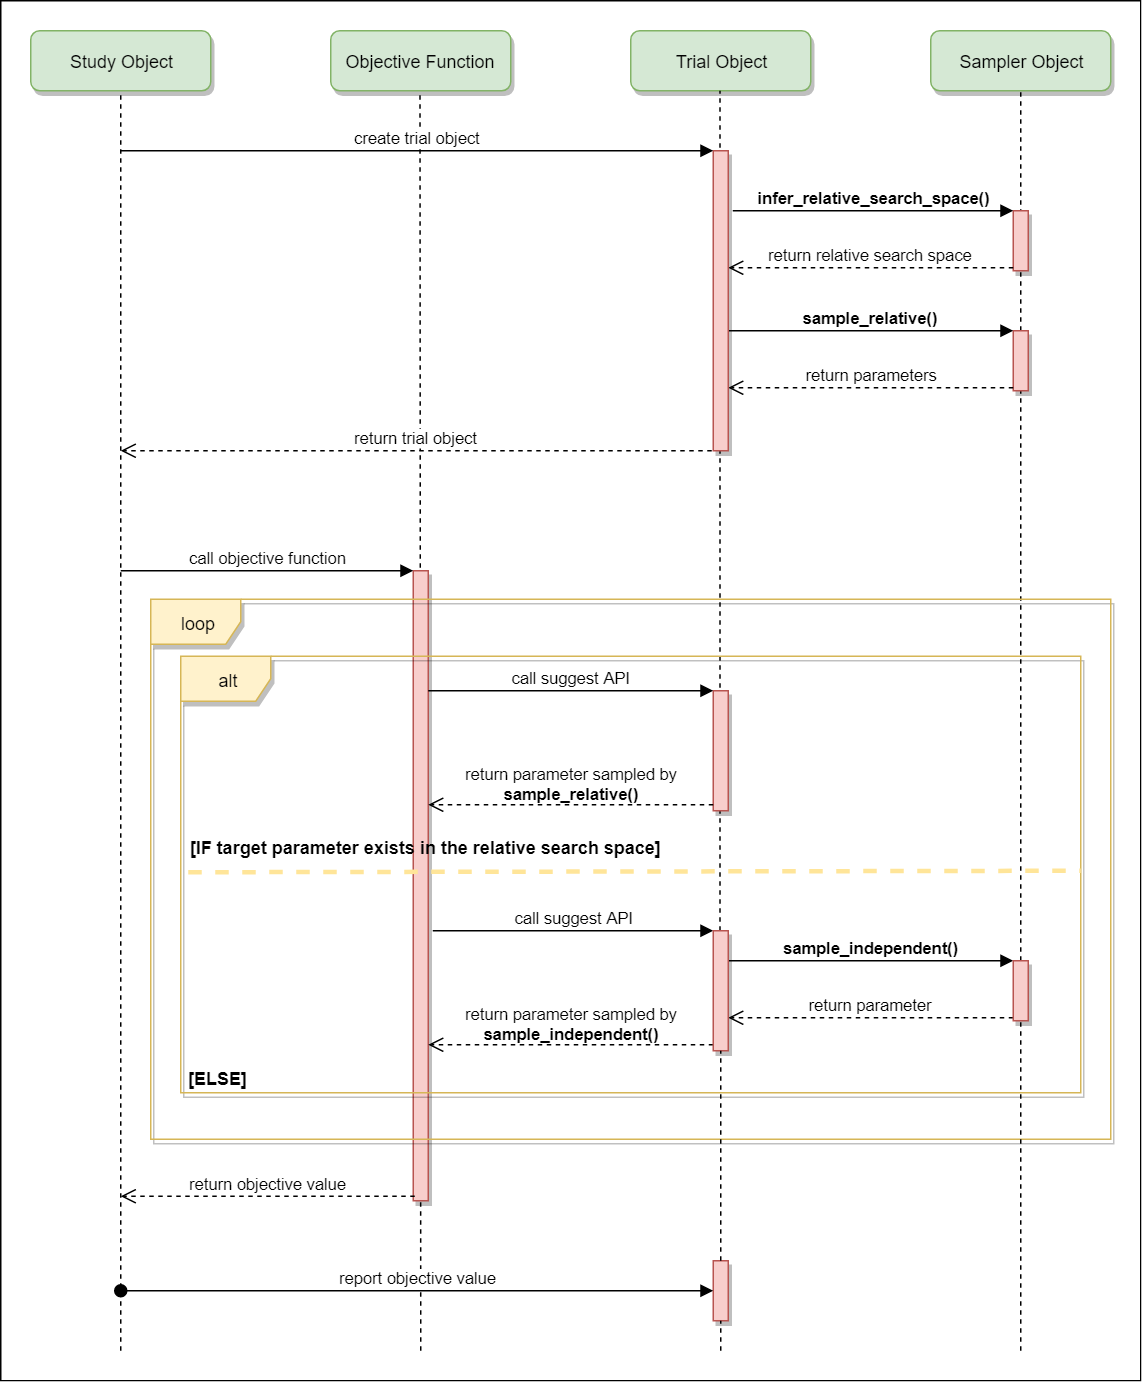
\includegraphics[width=15cm]{figures/figure-3.3.2.png}
	\caption[Sequence Diagram of Optuna's Samplers]{Sequence Diagram of the interaction between Optuna's Samplers and the rest of the Optuna's components. Through the diagram, is possibile to understand how a sampler in Optuna behaves at the start of a Trial. Source: \cite{Optuna}}
	\label{fig:figure-3.3.2}
\end{figure}
% \begin{figure}[t]
% 	\centering
% 	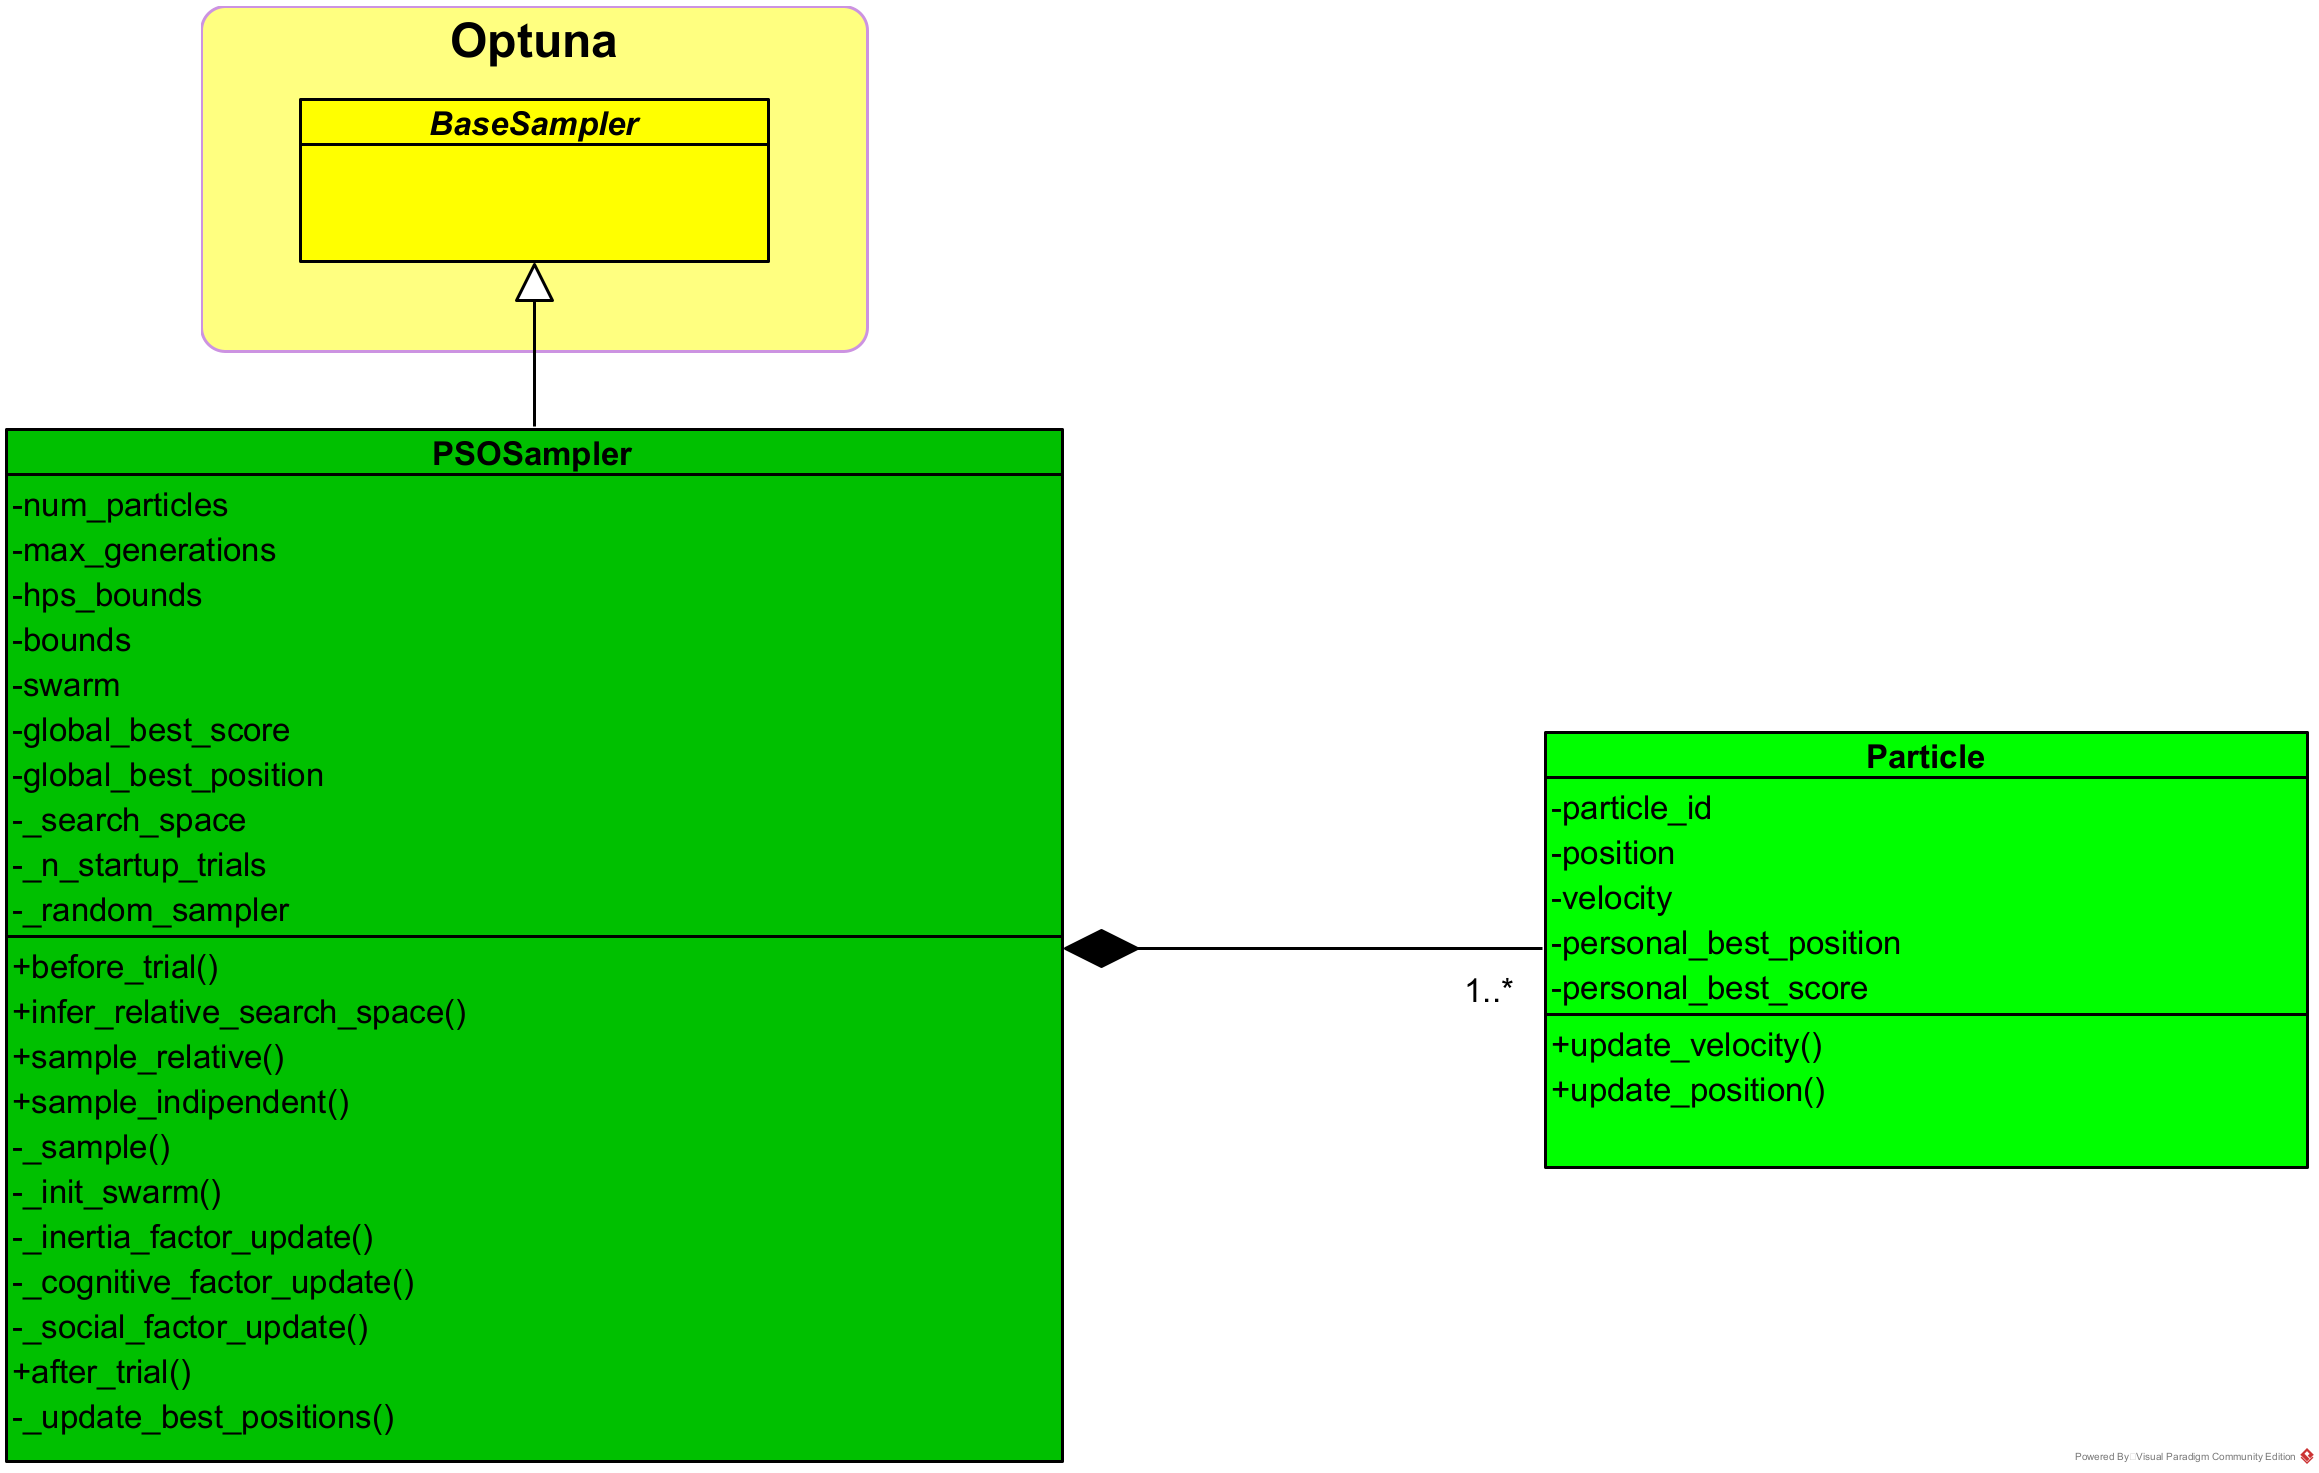
\includegraphics[width=15cm]{figures/figure-3.3.3.png}
% 	\caption[Class Diagram of PSOSampler]{Class Diagram of the implementation of the PSOSampler.}
% 	\label{fig:figure-3.3.3}
% \end{figure}

\subsubsection{Sampling}

At the start of each Trial, the \texttt{before\_trial()} method is called. There, depending on its number, a specific Particle and the current generation are assigned to the Trial.
\\[0.3cm]The Sampling of each candidate tuple of Hyperparameters happens through the \newline\texttt{sample\_relative()} method, which after checking what Particle the current Trial refers to, gets the position of the Particle and converts its coordinates into HPs values.

\subsubsection{After Trial}

At the end of each trial, the \texttt{after\_trial()} method is called.
The Particle associated with the Trial is updated; the values for $w$, $c_1$ and $c_2$ are obtained in the same way described in the section on Custom Implementation of PSO (Sec.~\ref{sec:CustomImplementationOfPSO-3.2}).
Local and Global best positions and scores are also checked and eventually updated.

\section{Applied Neural Network Models}

The type of Machine Learning model chosen for the experiment is Neural Networks.
The chosen library to implement the NN Models and the related support code (such as Loss Function, Train Loop) is PyTorch, which is the most popular Deep Learning library at the moment \cite{PyTorch}.
In the experiments, everything related to the architecture and to the training and evaluation of the models is implemented using PyTorch.

\subsection{Models}

In the experiments, two models have been used: MLP and Lawin.
\\[0.3cm]MLP, or Multi-Layer Perceptron, is the simplest type of Deep Learning Model. The implementation that was utilized is not the standard one of PyTorch but is a custom one, developed using PyTorch. The MLP is applied as the ML model for all the experiments except the last one.
\\[0.3cm]Lawin is a complex DL model specialized in Semantic Segmentation, it is applied only to the Weed Map experiment.

\subsubsection{MLP}

This implementation of the MLP simply follows the standard characteristics of the basic form of MLP (Fig.~\ref{fig:figure-3.4.1}).
Its architecture is represented by a list of values, where the length of the list is the Depth of the Hidden Layer, and the value in the list is the Width of the Layer at the corresponding index.
Both the Architecture and the Activation Function are initialization inputs.
\begin{figure}[t]
	\centering
	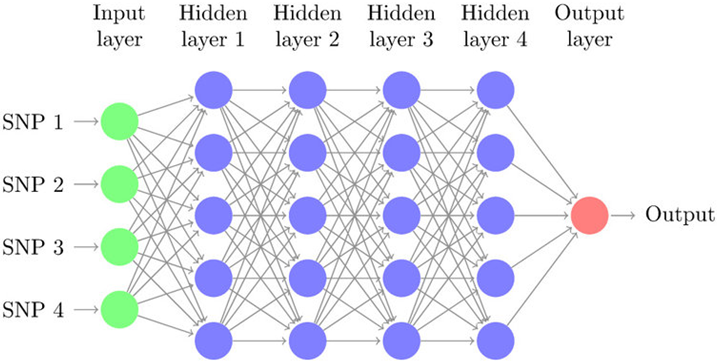
\includegraphics[width=10cm]{figures/figure-3.4.1.png}
	\caption[Visual Example Representation of MLP]{Visual representation of a MLP Neural Network. In this specific example, the input layer consists of four neurons, the output layer of just one, and each hidden layer of five; the width of the hidden part of the network is in this case four. Source: Google Images}
	\label{fig:figure-3.4.1}
\end{figure}
\\[0.3cm]This implementation of MLP refers to the file \texttt{/utils/model/MLP.py} of the code repository \cite{Repository-THESIS}.

\subsubsection{Lawin}\label{sec:Lawin-3.4.1.2}

Lawin is a complex Deep Learning model, in particular is a Vision Transformer, specialized in Semantic Segmentation and applied to Drone Vision problems.
Lawin was developed for this article \cite{WeedMap-PaperThesis}, and its implementation can be found in the relative repository \cite{WeedMap-Repository}.
% 
% \myparagraph{Architecture of Lawin:}
\\[0.3cm]Lawin consists of an Encoder and a Decoder (Fig.~\ref{fig:figure-3.4.2}).
The encoder is a Mix Transformer (MiT), which can generate CNN-like multi-level features with different resolutions, providing a feature map for each Transformer block as output.
The decoder uses a Large Window Attention Spatial Pyramid Pooling (LawinASPP), consisting of five parallel branches, a pooling layer, a shortcut connection, and three large window attentions with different context sizes.
\begin{figure}[t]
	\centering
	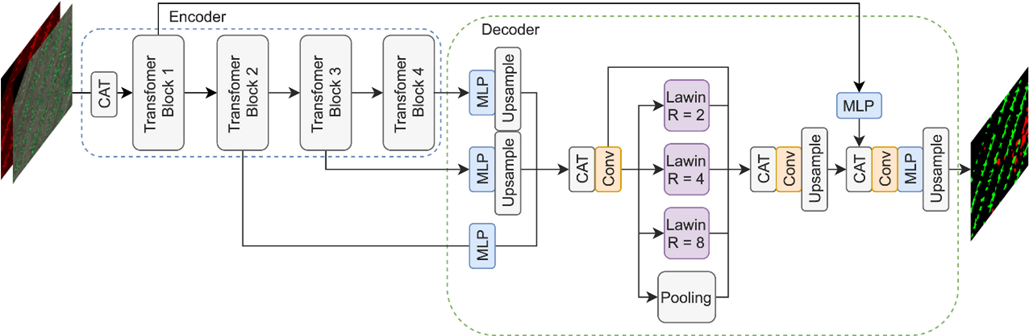
\includegraphics[width=15cm]{figures/figure-3.4.2.png}
	\caption[Architecture of Lawin]{Architecture of Lawin. Source: \cite{WeedMap-PaperThesis}}
	\label{fig:figure-3.4.2}
\end{figure}
% 
% \myparagraph{Variants of Lawin:}
\\[0.3cm]Variants of Lawin are: Double Lawin and Split Lawin.
Those variants are mentioned in this article \cite{WeedMap-PaperThesis} but are not utilized in any of the proposed experiments.

\subsection{Loss Functions}

In Neural Networks, during the training process, the Loss Function calculates the distance between the prediction of the model and the actual target value.
\\[0.3cm]In the experiments, two loss functions have been used, which are Cross Entropy and Focal.
For the Weed Map experiment only FocalLoss has been used, whereas both (or sometimes only CrossEntropyLoss) have been used for all other experiments.
\\[0.3cm]\texttt{CrossEntropy} is the implementation from PyTorch, the one inside the package \texttt{nn}. \texttt{FocalLoss} is implemented with PyTorch.

\subsubsection{Cross Entropy Loss}

Cross Entropy Loss, a loss function principally applied in classification problems, measures the difference between two probability distributions: the true distribution (actual labels) and the predicted distribution (model outputs).
Basically, it determines how far the model's predictions are from the labels (the targets).

\subsubsection{Focal Loss}

Focal Loss is an extension of Cross Entropy Loss. This particular implementation of Focal Loss is from the same article and repository mentioned in the previous sections about Lawin \cite{WeedMap-PaperThesis} \cite{WeedMap-Repository}.
Focal Loss is calculated as follows:
\begin{equation}
	FL=-w_c (1-f(x)_c ) log(f(x)_c)
\end{equation}
In the formula, $f(x)_c$ is the probability of the true class predicted by the model, and $w_c$ is the corresponding class weight.
An interpretation of this formula is that different weights are given to different classes of the classification task. This is to address the class imbalance, particularly in scenarios where some classes are significantly more frequent than others.
\\[0.3cm]A more detailed explanation of Focal Loss is in the earlier mentioned article \cite{WeedMap-PaperThesis}. The original form of Focal Loss was presented in this other article \cite{FocalLoss}.

\subsection{Training and Evaluation}

The functions to train and evaluate the models are also written using PyTorch.
\\[0.3cm]All the code mentioned in this section refers to the package \texttt{/utils/training} of the code repository \cite{Repository-THESIS}. The three illustrated files are \texttt{eval\_step.py}, \texttt{train\_step.py}, and \texttt{train\_loop.py}.

\subsubsection{Training Step}

In the \texttt{train\_step()} function, the PyTorch model is set in Training Mode, and the backward step is executed, calculating the gradients.
Basically, this Training Step is the training loop within a single Epoch.

\subsubsection{Evaluation Step}

In the \texttt{eval\_step()} function the PyTorch model is set in Evaluation Mode, then predictions are made using the validation or test data loaders and compared with the target values.
The performance is evaluated using a specific Metric. In order for this code to be as abstract as possible, a class called \texttt{MetricWrapper} (defined in the \texttt{/utils/metrics} package) was implemented, which abstracts the methods of initialization, computing, and value return of the metrics.
\\[0.3cm]All four main evaluation metrics are calculated (Accuracy, Precision, Recall, F1), but only one is considered toward the final score of the evaluation. The chosen metric is F1 for the Weed Map experiment and Accuracy for all other experiments.

\subsubsection{Training Loop}

In the \texttt{full\_train\_loop()} function, the PyTorch model is fully trained, iterating over the maximum number of epochs, and executing \texttt{train\_step()} and \texttt{eval\_step()} at each iteration.
The function also contains instructions related to pruning, early stopping, logging, and data persistence.

\subsection{Regularization}

Regularization is a technique used to prevent overfitting in Neural Networks. More generally, it is a technique that can be used in multi-objective optimization, to penalize certain characteristics of a candidate solution by lowering its score.
\\[0.3cm]In the proposed experiments, the Regularization technique has the goal of penalizing the complexity of the model, in terms of the width and depth of the hidden layers. Basically, a penalty term is applied referring to the complexity of the model's architecture.
\\[0.3cm]In the experiments, as all of them share a secondary objective to reduce the complexity of the found solutions, a penalization toward architecture complexity was applied. Whenever “Score” is mentioned, it refers to the regularized score, rather than the specific metric score (Accuracy or F1). Which is calculated as follows:
\begin{equation}
	Score = ms - \lambda \cdot complexity
\end{equation}
In the formula: $ms$ is the metric score (could be Accuracy or F1), $\lambda$ (\texttt{lambda}) is the Regularization coefficient (which is passed as input) and $complexity$ is the complexity of the model, which is calculated as the sum of the number of neurons in each hidden layer.
\\[0.3cm]The Regularization was implemented with a \texttt{Regularizer} class defined in the\newline\texttt{/utils/optimization/regularizer.py} file of the code repository \cite{Repository-THESIS}.

\subsection{Other Training-Related Objects}

Inside the \texttt{/utils/model/model\_utils.py} file of the code repository \cite{Repository-THESIS} are defined other aspects of the training process of the model, such as the initialization of Activation Functions and Optimizers.
\\[0.3cm]The possible Activation Functions are Sigmoid, ReLU and Softmax. The \newline\texttt{get\_activation\_fn()} function takes as an input the string sampled from Optuna representing one Activation Function and returns the initialized corresponding object using the PyTorch implementation.
\\[0.3cm]The possible Optimizers are SGD (Stochastic Gradient Descent) and ADAM. The \texttt{get\_optimizer()} function takes as an input the string sampled from Optuna representing one Optimizer and returns the initialized corresponding object using the PyTorch implementation.



